\section{Probability and Randomness}\label{sec:prob}

In mathematics, the word ``random'' has a more precise meaning than in everyday 
speech. Something is random if its outcome is governed by what's called a 
\emph{probability distribution}. 
For example, the outcome $c$ of a coin toss is not fixed, but takes 
on one of the values in the set $\{H, T\}$, where $H$ means heads and $T$ means 
tails. (This is called the \emph{sample space} of $c$.) We write 
that $c \in \{H,T\}$, where the symbol $\in$ is read aloud as 
``is an element of'' or simply ``is in''.
The value of $c$ is described by the distribution $\left\{\frac{1}{2}, 
\frac{1}{2}\right\}$ \new{over the set $\{H,T\}$}, meaning each outcome ($H$ or $T$) happens with 
probability one-half.

\begin{example}\label{ex:prob-dist}
    Here are some other everyday probability distributions and their 
    sample spaces:
    \renewcommand{\labelenumi}{(\alph{enumi})} 
    \begin{enumerate}
        \item The probability distribution of phone type used by Americans 
        in 2021 over the sample space \{Android, iPhone, Other\} is $\{44.0\%\footnotemark[1],
        46.9\%\footnotemark[2],9.1\%\}$.
        \footnotetext[1]{
            \url{https://www.statista.com/statistics/201182/forecast-of-smartphone-users-in-the-us/},
            \url{https://www.statista.com/statistics/232786/forecast-of-andrioid-users-in-the-us/}
        }
        \footnotetext[2]{
            \url{https://www.statista.com/statistics/236550/percentage-of-us-population-that-own-a-iphone-smartphone/}
        }
        \item The distribution over the outcomes of a dice roll $\{1,2,3,4,5,6\}$
        is $\{\frac{1}{6},\frac{1}{6},\frac{1}{6},\frac{1}{6},\frac{1}{6},\frac{1}{6}\}$.
    \end{enumerate}
\end{example}

\begin{exercise}
    Write the sample space and probability distribution of each of 
    the following random variables:
    \renewcommand{\labelenumi}{(\alph{enumi})} 
    \begin{enumerate}
        \item Card drawn from a shuffled deck.
        \item Registration status of students at a 2000-person high school 
        where all but 100 students register for classes every year.
    \end{enumerate}
\end{exercise}

A variable like $c$ that represents an outcome or event is called a \emph{random 
variable}, since it can take on one of several values based on an underlying 
probability distribution. A random variable is \emph{uniformly random} if every possible 
value is equally likely. We call this probability distribution the 
\emph{uniform distribution}. The variable $c$ is uniformly random (or simply \emph{uniform})
since $H$ and $T$ occur with equal probability, namely both with probability 
$\frac{1}{2}$. \new{We say such a variable is ``chosen uniformly at random'' 
(sometimes shortened to ``chosen uniformly'') and denote this with the symbol 
$\sample$. For instance, the coin toss example is written as $c \sample \{H, T\}$, 
meaning that $c$ is sampled uniformly from the set $\{H, T\}$.}

% \new{Additionally, we can abbreviate the uniform probability distribution 
% over $\{H,T\}$ as $U(H,T)$, where the $U$ stands for ``uniform''. \todo{since 
% there are two elements in the parentheses, it's implied that each has probability 
% $\frac{1}{2}$.}
% This is especially useful in cases like part (b) of Example~\ref{ex:prob-dist},
% where we can write the distribution much more compactly as $U(1,2,3,4,5,6)$.}

\begin{exercise}
    Write ``uniform'' or ``not uniform'' for each of the following random variables:
    \renewcommand{\labelenumi}{(\alph{enumi})} 
    \begin{enumerate}
        \item Drawing a card from the top of a shuffled deck.
        \item Drawing a card from the top of an ordered deck.
        \item The weather on a given day.
        \item The outcome of a dice roll.
        \item The birthday of the first person you encounter on the street.
    \end{enumerate}
\end{exercise}

\begin{exercise}
    How would you represent a dice roll using the $\sample$ notation?
\end{exercise}

We use $\Pr$ to denote the probability of some event. For instance, the 
probability that $c$ is heads is one-half. In mathematical notation this
is written as
\[
    \Pr[c=H] = \frac{1}{2}
\]
Similarly, $c$ is tails with probability one-half:
\[
    \Pr[c=T] = \frac{1}{2}
\]

Given these two facts, what is the probability of getting heads \emph{or}
tails? Because these two events are \emph{mutually exclusive} (that is, 
if one occurs, it means the other cannot possibly have occured, and 
vice versa), we can add their probabilities:
\begin{align*}
    \Pr[c = H \text{ or } T] &= \Pr[c=H] + \Pr[c=T] \\
    &= \frac{1}{2} + \frac{1}{2} = 1
\end{align*}

Notice that these probabilities sum to 1. 
This is a common requirement of all probability distributions: the sum of their 
probabilities must be 1. This is the same as saying that \emph{one of} the possible events 
in the distribution happens with 100\% probability. If the sum was less than 1, it 
would mean that there's some other event that could happen instead, so the distribution
is incomplete. % If it was greater than 1, then the 

The pie charts below illustrate this idea. On the left is the probability 
distribution of a coin toss; on the right, the probability distribution 
of a dice roll. Notice that in both cases, the probabilities sum to 1.

\begin{figure}[h]
    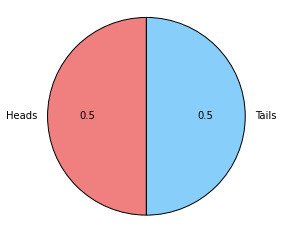
\includegraphics[width=.5\linewidth]{imgs/coin-pie.png}
    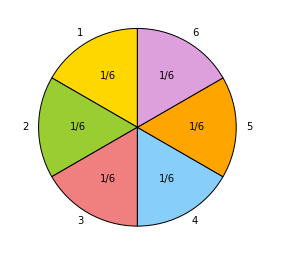
\includegraphics[width=.5\linewidth]{imgs/die-pie.png}
    % \caption{Left: probability distribution of a coin toss. Right: 
    % probability distribution of a dice roll. Probabilities always 
    % sum to 1.}
    \label{fig:pies}
  \end{figure}

When two events are not mutually exclusive, however, we can't add 
their probabilities. For example, what's the probability of rolling a 
multiple of 2 or a multiple of 3? These are not mutually exclusive
events, since 6 is a multiple of \emph{both} 2 and 3! Instead, we need 
to break this question into mutually exclusive events. We could consider 
the probability of rolling a multiple of two, and add this to the 
probability of rolling a 3: by doing this, we still cover all the 
possible outcomes (2, 3, 4, and 6) but broken into mutually exclusive 
events ($\{2,4,6\}$ or $\{3\}$) instead of overlapping events ($\{2, 4, 
6\}$ or $\{3, 6\}$). Then

\begin{align*}
    &\Pr[d \text{ is a multiple of 2 or 3}] \\
    &= \Pr[d \text{ is even}] + \Pr[d=3]\\
    &= \frac{1}{2} + \frac{1}{6}\\
    &= \frac{4}{6} = \frac{2}{3}
\end{align*}

where $d$ is the random variable representing the outcome of the die roll.

\hfill\\

Conditional probability is the probability that something occurs 
provided that another event occurred. This is written with the symbol 
$\mid$, which is read aloud as ``given''. So, $\Pr[A \mid B]$ is 
read as ``the probability of $A$ given $B$''.

For example, it's more likely to be raining if the sky is cloudy 
than if it's clear. We can write this as
\[
    \Pr[\text{raining} \mid \text{cloudy sky}] >
    \Pr[\text{raining} \mid \text{clear sky}]
\]

The following equality about conditional probability always holds\footnotemark:
\footnotetext{With the caveat is that we cannot condition on a zero-probability
event (that is, we require $\Pr[B] \neq 0$) since we cannot divide by zero.}
\begin{subequations}\label{eq:conditional}
    \begin{equation}
        \Pr[A \mid B] = \frac{\Pr[A \text{ and } B]}{\Pr[B]}
        \label{eqn:conditional_mid}
    \end{equation}
An alternate form is
    \begin{equation}
        \Pr[A \text{ and } B] = \Pr[A \mid B] \cdot \Pr[B]
        \label{eqn:conditional_and}
    \end{equation}
\end{subequations}

Understanding why these equations are true can help us remember them.
One way to see why they hold is with a Venn diagram:

\begin{center}
\begin{tikzpicture}
    % A
    \node[draw,%anchor=west,
        circle,minimum size=5cm,
        % label={0:$A$},
        ]                           (A) at (0,0) {};
    % B
    \node[draw,%anchor=east,
        pattern=north east lines,
        fill opacity=0.5,
        circle,minimum size=5cm,
        % label={45:$B$},
        ]                           (B) at (3,0) {};
    % labels
    \node                               at (1.5,0) {$A$ and $B$};
    \node                               at (-1,0) {$A$ happened};
    \node                               at (4,0) {$B$ happened};

    \begin{scope}
        \clip (0,0) circle(2.5cm);
        \clip (3,0) circle(2.5cm);
        \fill[pattern=north west lines,
            opacity=0.5
            ]                       (0,0) circle(2.5cm);
    \end{scope}
\end{tikzpicture}
\end{center}

Let's think through Equation~\ref{eqn:conditional_mid} with this diagram 
in front of us. The event ``$A$ given $B$'' means we know $B$ happened, 
so now our entire realm of possibilities exists only in the circle 
on the right. Let's zoom in on that circle:

\begin{center}
\begin{tikzpicture}
    % B
    \node[draw,%anchor=east,
        circle,minimum size=5cm,
        % label={45:$B$},
        ]                           (B) at (0,0) {};
    % labels
    \node[align=right]                        at (1.1,0) {all possible\\events};
    \node                                     at (-1.5,0) {$A$};

    \begin{scope}
        \clip (0,0) circle(2.5cm);
        \draw (-3,0) circle(2.5cm);
    \end{scope}
    \begin{scope}
        \clip (0,0) circle(2.5cm);
        \clip (-3,0) circle(2.5cm);
        \fill[pattern=north west lines,
            opacity=0.5
            ]                       (0,0) circle(2.5cm);
    \end{scope}
\end{tikzpicture}
\end{center}

The cases in which $A$ happens next are in the little slice on the 
left. We want to know the probability $A$ happening given our current 
information, which is simply the fraction of possible events covered by 
this area. Zooming back out, that's exactly $\Pr[A \text{ and } B]$ 
divided by $\Pr[B]$!

The difference is the reference frame: in the first diagram, we are in a 
world in which we make no assumptions: all possibilities are open. In 
the second, we are using the extra information that $B$ happened to 
limit the world of possibilities. Let's see some concrete examples next.

\begin{example}\label{ex:cond-vis}
    Consider the following sample space, where each number is chosen with 
    equal probability.
    Throughout the example, let $B = \{3,4,7,8,11,12,15,16\}$ (the shaded 
    cells).

    \begin{center}
    \begin{tikzpicture}
        \draw(0,0) grid (4,4);
        \node at (0.5,3.5) {1};
        \node at (1.5,3.5) {2};
        \node at (2.5,3.5) {3};
        \node at (3.5,3.5) {4};
        \node at (0.5,2.5) {5};
        \node at (1.5,2.5) {6};
        \node at (2.5,2.5) {7};
        \node at (3.5,2.5) {8};
        \node at (0.5,1.5) {9};
        \node at (1.5,1.5) {10};
        \node at (2.5,1.5) {11};
        \node at (3.5,1.5) {12};
        \node at (0.5,0.5) {13};
        \node at (1.5,0.5) {14};
        \node at (2.5,0.5) {15};
        \node at (3.5,0.5) {16};
        \filldraw[pattern=north east lines,opacity=0.5] (2,0) rectangle (4,4);
        \node at (3,4.5) {$B$};
    \end{tikzpicture}
    \end{center}

    Notice that $\Pr[B] = \frac{8}{16} = \frac{1}{2}$.
    

    \renewcommand{\labelenumi}{(\alph{enumi})} 
    \begin{enumerate}
        \item Suppose $A = \{9,10\}$:
            \begin{center}
            \begin{tikzpicture}
                \draw(0,0) grid (4,4);
                \node at (0.5,3.5) {1};
                \node at (1.5,3.5) {2};
                \node at (2.5,3.5) {3};
                \node at (3.5,3.5) {4};
                \node at (0.5,2.5) {5};
                \node at (1.5,2.5) {6};
                \node at (2.5,2.5) {7};
                \node at (3.5,2.5) {8};
                \node at (0.5,1.5) {9};
                \node at (1.5,1.5) {10};
                \node at (2.5,1.5) {11};
                \node at (3.5,1.5) {12};
                \node at (0.5,0.5) {13};
                \node at (1.5,0.5) {14};
                \node at (2.5,0.5) {15};
                \node at (3.5,0.5) {16};
                \filldraw[pattern=north east lines,opacity=0.5] (2,0) rectangle (4,4);
                \filldraw[pattern=north west lines,opacity=0.5] (0,1) rectangle (2,2);
                \node at (3,4.5) {$B$};
                \node at (-0.5,1.5) {$A$};
            \end{tikzpicture}
            \end{center}

            Since $A$ and $B$ don't overlap, $\Pr[A \text{ and } B] = 0$. 
            Then, using Equation~\ref{eqn:conditional_mid}, $\Pr[A \mid B] 
            = \Pr[A \text{ and } B] \div \Pr[B] = 0 \div \frac{1}{2} = 0$.
            Using the visual intuition we gained with the Venn diagrams, 
            we can justify this by saying that $A$ occupies 0 of the space
            of $B$.

        \item Now let $A = \{10,11\}$:
            \begin{center}
            \begin{tikzpicture}
                \draw(0,0) grid (4,4);
                \node at (0.5,3.5) {1};
                \node at (1.5,3.5) {2};
                \node at (2.5,3.5) {3};
                \node at (3.5,3.5) {4};
                \node at (0.5,2.5) {5};
                \node at (1.5,2.5) {6};
                \node at (2.5,2.5) {7};
                \node at (3.5,2.5) {8};
                \node at (0.5,1.5) {9};
                \node at (1.5,1.5) {10};
                \node at (2.5,1.5) {11};
                \node at (3.5,1.5) {12};
                \node at (0.5,0.5) {13};
                \node at (1.5,0.5) {14};
                \node at (2.5,0.5) {15};
                \node at (3.5,0.5) {16};
                \filldraw[pattern=north east lines,opacity=0.5] (2,0) rectangle (4,4);
                \filldraw[pattern=north west lines,opacity=0.5] (1,1) rectangle (3,2);
                \node at (3,4.5) {$B$};
                \node at (-0.5,1.5) {$A$};
            \end{tikzpicture}
            \end{center}

            Now exactly one number, 11, is in both $A$ and $B$, so $\Pr[A \text{ and } 
            B] = \frac{1}{16}$. Thus $\Pr[A \mid B] = \frac{1}{16} \div \frac{1}{2}
            = \frac{1}{8}$. Visually, we notice that $A$ in fact occupies one-eighth
            of $B$'s space.

        \item Lastly, let $A = \{11,12\}$:
            \begin{center}
            \begin{tikzpicture}
                \draw(0,0) grid (4,4);
                \node at (0.5,3.5) {1};
                \node at (1.5,3.5) {2};
                \node at (2.5,3.5) {3};
                \node at (3.5,3.5) {4};
                \node at (0.5,2.5) {5};
                \node at (1.5,2.5) {6};
                \node at (2.5,2.5) {7};
                \node at (3.5,2.5) {8};
                \node at (0.5,1.5) {9};
                \node at (1.5,1.5) {10};
                \node at (2.5,1.5) {11};
                \node at (3.5,1.5) {12};
                \node at (0.5,0.5) {13};
                \node at (1.5,0.5) {14};
                \node at (2.5,0.5) {15};
                \node at (3.5,0.5) {16};
                \filldraw[pattern=north east lines,opacity=0.5] (2,0) rectangle (4,4);
                \filldraw[pattern=north west lines,opacity=0.5] (2,1) rectangle (4,2);
                \node at (3,4.5) {$B$};
                \node at (4.5,1.5) {$A$};
            \end{tikzpicture}
            \end{center}

            Now $\Pr[A \text{ and } B] = \frac{2}{16} = \frac{1}{8}$, so $\Pr[A \mid B]
            = \frac{1}{8} \div \frac{1}{2} = \frac{1}{4}$. Again, this makes 
            sense visually as well, since $A$ occupies one-quarter of $B$.
    \end{enumerate}
\end{example}

\begin{example}
    Suppose your friend rolls a die without showing you the result.
    You know the probability that they rolled a 3 is $\frac{1}{6}$. Now 
    suppose they tell you, ``I rolled an odd number.'' Using this additional 
    information, you can update your estimate of the probability that the 
    die roll is a 3 to $\frac{1}{3}$, since you know the die landed with 
    equal probability on 1, 3, or 5, and definitely didn't land on 2, 4, 
    or 6.

    Written in the language of conditional probability, this is
    \begin{align*}
        \Pr[d = 3 \mid d \text{ is odd}] 
        &= \frac{
                \Pr[d=3 \text{ and } d \text{ is odd}]
            }{
                \Pr[d \text{ is odd}]
            }\\
        &= \frac{
                \Pr[d=3]
            }{
                \Pr[d \text{ is odd}]
            }\\
        &= \frac{1}{6} \div \frac{1}{2} = \frac{2}{6} = \frac{1}{3}
    \end{align*}
\end{example}

\begin{exercise}
    Repeat Example~\exref{ex:cond-vis}, calculating $\Pr[B \mid A]$ instead.
\end{exercise}

In some cases, such as Example~\exref{ex:cond-vis}b, we have $\Pr[A \mid 
B]=\Pr[A]$. Intuitively, this means 
that the probability of $A$ is the same regardless of whether or not $B$
happened. For example, a good coin toss should be independent of the coin 
used for the toss or the person doing the toss.
In these cases, we say that $A$ and $B$ are \emph{independent} events, and 
their corresponding random variables are independent. Then Equation~\ref{eqn:conditional_and}
simplifies to 
\begin{equation}\label{eq:and}
   \Pr[A \text{ and } B] = \Pr[A] \cdot \Pr[B]
\end{equation}
This means that for independet random variables, we can just multiply the probabilities 
of two events together to get the probability that both events happen simultaneously.

\begin{example}
    Suppose I roll a die and flip a coin. What's the probability that I roll a 1 
    \emph{and} get heads?

    Our first instinct might be to list out all of the possible 
    combinations of events; for each outcome of the roll, there is a tails and a 
    heads option:

    \[
        1H, 1T, 2H, 2T, 3H, 3T, 4H, 4T, 5H, 5T, 6H, 6T
    \]

    Each of these outcomes occurs with equal probability, and there 
    are twelve of them, so rolling a 1 and getting heads ($1H$) occurs 
    with probability $\frac{1}{12}$.

    If we realize that the dice and coin outcomes are independent, however,
    we can get to this answer in a simpler way. Looking at Equation~\ref{eq:and}, 
    we see that we can multiply the probabilities of the two events together
    the get the probability of \emph{both} events occuring. Let 
    $d$ be the random variable representing the outcome of the die roll and $c$ 
    be the random variable representing the outcome of the coin toss. Then 

    \begin{align*}
        &\Pr[d=1 \text{ and } c=H]\\
        =& \Pr[d=1] \cdot \Pr[c=H]\\
        =& \frac{1}{6} \cdot \frac{1}{2} = \frac{1}{12}
    \end{align*}
\end{example}

\begin{exercise}
    Suppose I flip two coins. What's the probability of both coins landing on heads?
\end{exercise}

Let's put everything we've learned so far together and work through some examples. 
Remember, for the \textbf{or} of two mutually exclusive events, we add; 
for the \textbf{and} of two independent events, we multiply. In the latter 
case, if the events aren't mutually exclusive, we use conditional probability 
(Equations~\ref{eqn:conditional_mid} and~\ref{eqn:conditional_and}).

\begin{example}
    Say I flip a fair coin twice. What's the probability of getting the 
    same result both times?

    There are two ways of getting the same result on both flips: we either 
    get heads twice (HH) or tails twice (TT):
    \[
        \Pr[HH] + \Pr[TT]
    \]

    Because subsequent coin flips are independent of each other, this is equal to 
    \[
        \Pr[H]\cdot \Pr[H] + \Pr[T]\cdot\Pr[T]
    \]

    Since the coin is fair, each outcome (heads or tails) happens with equal 
    probability, so this equals
    \begin{align*}
        & \frac{1}{2}\cdot\frac{1}{2} + 
        \frac{1}{2}\cdot\frac{1}{2}\\
        =& \frac{1}{4} + \frac{1}{4}\\
        =& \frac{1}{2}
    \end{align*}
\end{example}

\begin{exercise}
    Suppose I only flip a coin again if my first coin toss came out tails. 
    What's the probability of getting one heads outcome?
\end{exercise}

\begin{exercise} The following questions deal with rolling a 6-sided die.
    \renewcommand{\labelenumi}{(\alph{enumi})} 
    \begin{enumerate}
        \item What's the probability of rolling an even number?
        \item What's the probability of rolling a 1 followed immediately by a 2?
        \item If I roll twice, what's the probability that my second roll will 
        be higher than my first?
        \item Suppose that when I roll a 1, I get to reroll and use the 
        second number instead. What's the probability of rolling a 5 or higher?
    \end{enumerate}
\end{exercise}

When two random variables have the same underlying probability 
distribution, we say they are \new{\emph{perfectly indistinguishable}. 
For example, if $d_1 \in \{1,2,3,4,5,6\}$ is the random variable 
representing the outcome of rolling a 6-sided die, the probability 
distribution of $d_1$ is}
\begin{align*}
    \color{blue}
    \left\{
        \frac{1}{6},\frac{1}{6},\frac{1}{6},
        \frac{1}{6},\frac{1}{6},\frac{1}{6}
    \right\}
\end{align*}
\new{where each probability is the probability that $c$ takes on the 
corresponding value in the sample space.}

\new{Let's compare this to rolling a 12-sided die and dividing the result 
by 2, rounding up to the nearest whole number. That is, if we roll a 
1 or 2 on the die, the result is 1, if we roll a 3 or 4, the result 
is 2, and so on.
Then the probability distribution over this random variable (call it 
$d_2$) is over the sample space $\{1,2,3,4,5,6\}$, with values }
\begin{align*}
    \color{blue}
    \left\{
        \frac{1}{6},\frac{1}{6},\frac{1}{6},
        \frac{1}{6},\frac{1}{6},\frac{1}{6}
    \right\}
\end{align*}
\new{The sample space is the same in both cases, and each outcome in that sample
space occurs with the same probability in both distributions. So they're
the same distribution! Therefore $d_1$ and $d_2$ are perfectly indistinguishable.}

% \todo{For example,
% if $c \in \{HHH, HHT,\allowbreak HTH, HTT, THH, THT, TTH, TTT\}$ 
% is the random variable representing the outcome of three coin tosses,
% the probability distribution of $c$ is }
% \begin{align*}
%     \color{red}
%     \left\{
%         \frac{1}{8},\frac{1}{8},\frac{1}{8},\frac{1}{8},
%         \frac{1}{8},\frac{1}{8},\frac{1}{8},\frac{1}{8}
%     \right\}
% \end{align*}

% \todo{where each probability is the probability that $c$ takes on the 
% corresponding value in the sample space.}

% \todo{Compare this to the probability distribution of the random 
% variable $d \in \{1,2,3,4,5,6,7,8\}$ for rolling an 8-sided die:}
% \[
%     \color{red}
%     \left\{
%         \frac{1}{8},\frac{1}{8},\frac{1}{8},\frac{1}{8},
%         \frac{1}{8},\frac{1}{8},\frac{1}{8},\frac{1}{8}
%     \right\}
% \]

% \todo{They're the same distribution! Therefore $c$ and $d$ are perfectly
% indistinguishable.}

\begin{exercise}
    Write ``perfectly indistinguishable'' or ``not perfectly indistinguishable''
    for each pair of probability distributions $D_1, D_2$:
    \renewcommand{\labelenumi}{(\alph{enumi})} 
    \begin{enumerate}
        \item $D_1$: Rolling an even or an odd number on a 6-sided die, 
        $D_2$: getting heads or tails when you flip a coin
        \item $D_1$: Drawing a random card from a shuffled deck, 
        $D_2$: rolling a 6-sided die and flipping 3 coins
        \item $D_1$: Whether or not you get at least one heads when flipping
        two coins, $D_2$: whether or not you draw a club from a shuffled 
        deck.
    \end{enumerate}
\end{exercise}

\subsection{Randomness in Cryptography}

As we'll see, randomness plays an extremely important role in modern cryptographic
schemes. A cryptographic \emph{scheme} is a well-defined procedure for accomplishing 
some \todo{blueprint with desirable properties} (called a \emph{cryptographic primitive}). For example, the Caesar 
cipher is an encryption scheme\footnotemark, meaning it is a procedure for accomplishing
the cryptographic primitive of encryption. 
In this packet, you'll learn about several \emph{secret sharing} schemes.
\footnotetext{Note, however, that it is \emph{not} a secure encryption scheme!
You can learn more about how the Caesar cipher works and its weakness 
here: \url{https://www.khanacademy.org/computing/computer-science/cryptography/crypt/v/caesar-cipher}.}

When a scheme's security rests only on the randomness used in it, and not on 
solving a difficult or very long problem, we say that scheme is
\emph{information-theoretically secure}. This is different from, for example,
the schemes in the RSA cryptography packet, whose security depends on 
the assumed difficulty of factoring\footnotemark.

\footnotetext{When a scheme is protected by how hard it is 
to compute something, it is said to be \emph{computationally secure}.}

\nsm{Not sure which security notion (perfect or statistical) I'm proving 
for the scheme later...}
\todo{The exact level of security of a scheme is determined by a \emph{security 
parameter}, which is a number that's often denoted by the symbol $\lambda$ 
(the Greek letter lambda). The people using a scheme will generally decide 
on the security parameter ahead of time based on how secure they want to
keep their information. 
There's usually a tradeoff between security and efficiency, so the 
parties will settle on a $\lambda$ that makes them feel safe enough without 
making their computations prohibitively slow (hours, days, or weeks).}
% We'll learn more about this in Section~\ref{sec:proof}.
% TODO: future version could have an example where lambda is too small 
% and show that an adversary can guess $s_1$ with non-negligible probability.

\todo{Lambda is usually set to a large power of two, like 128 or 256; to keep 
numbers reasonable in this packet, though, we'll let $\lambda=10$.}
